
% ----------------------------------------------------------
\begin{frame}
  \frametitle{Finding the Electron in Electronics}

  Transistor sizes from centimeters to nanometers
  
  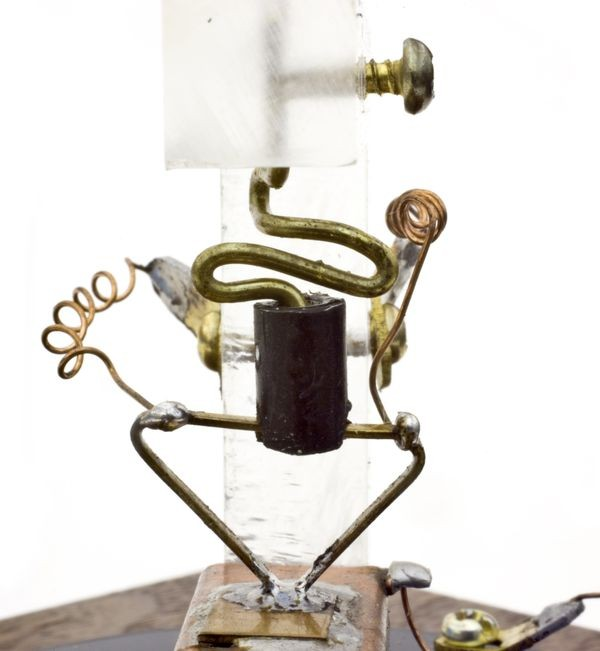
\includegraphics[width=0.2\linewidth]{Graphics/CHM-Transistor-picture.jpg}
  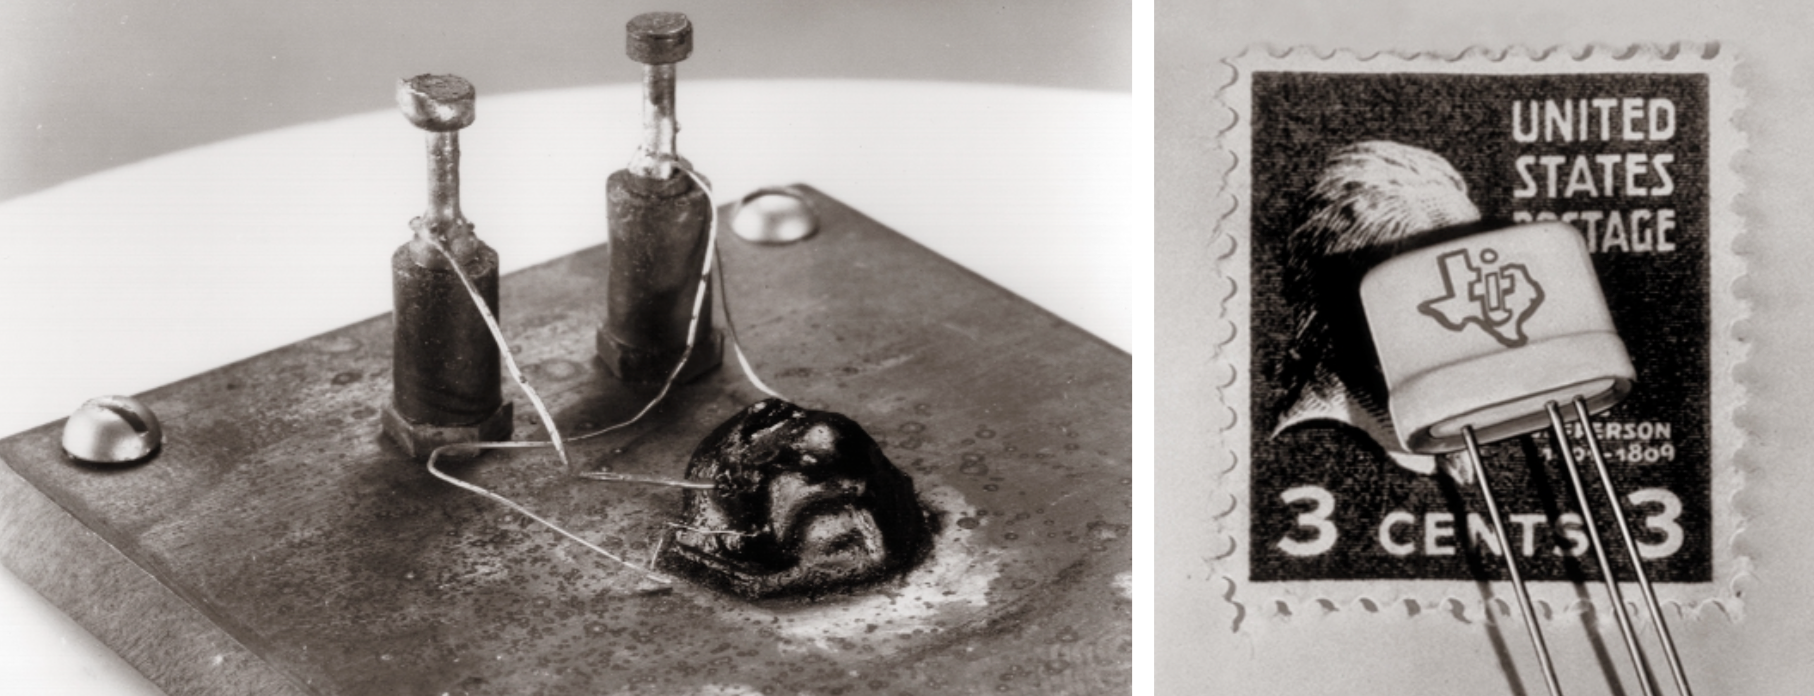
\includegraphics[width=0.35\linewidth]{Graphics/SE-Bell-junction.png}
  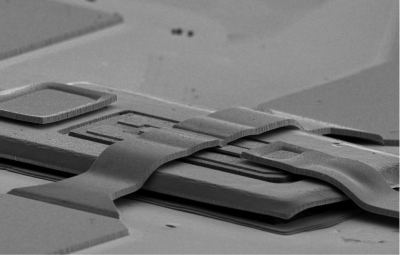
\includegraphics[width=0.20\linewidth]{Graphics/SE-bipolar-transistor.png}
  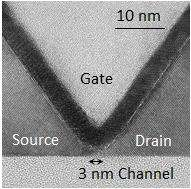
\includegraphics[width=0.20\linewidth]{Graphics/SE-3nm-channel-transistor.jpg}

  \begin{columns}
    % SET
    \column[T]{0.25\linewidth}
    Single electron transport (NIST)
  
    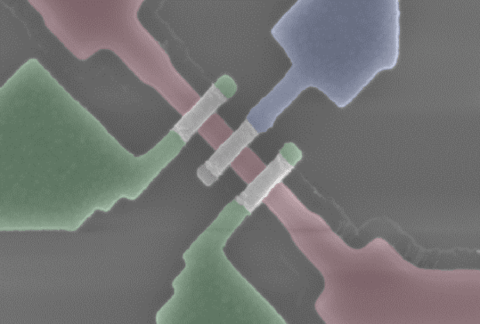
\includegraphics[width=0.95\linewidth]{Graphics/SE-NIST-set1.png}

    % electron angular momentum
    \column[T]{0.75\linewidth}
    \begin{block}{Hello Planck}
      orbit angular momentum of electron in lowest energy state of hydrogen
      is $\sqrt{2} \hbar$
    \end{block}
  \end{columns}

  images from various sources~\cite{CHM-Transistor-article, Lost-history-transistor, NRL-nanoelectronics,
    PhysOrg-3nm-channel-transistor, NIST-Single-electron-transport}
\end{frame}
